\section{Generalizirani ICP algoritam}
Eksperimantalni rezultati za generalizirajući algoritam iteracije točaka su prikazani u sljedećim tablicama i grafovima. Grafovi i tablice se odnose na podskupove točaka primjera A i B. Zbog fizičke ograničenosti računala ICP algoritam je izvršen na manjem skupu podataka.

\subsubsection{tavblica ekspreimentalnih rezultata}
\begin{table}[H]
  \begin{tabular}{ |p{3cm}| |p{2cm}|p{2cm}|p{2cm}|p{2cm}| }
    \hline
    Rezultati& Primjer 1& Primjer 2&Primjer 3& Primjer 4\\
    \hline
    AMx [$m$]& 0.18427& 2.7368e-3& 1.41374e-3& 3.63932e-2\\
    AMy [$m$]&  16.3356& 1.38002e-3& 2.8428e-3& 1.32941e-2\\
    AMz [$m$]& 0.01657& 4.02492e-3& 5.811e-4& 8.78942e-4\\
    AMr [$rad$]& 1.53082e-3& 9.69565e-5& 4.95289e-5& 1.44264e-4\\
    AMp [$rad$]& 6.81777e-3& 8.68708e-5& 3.69849e-4& 2.43620e-4\\
    AMy [$rad$]& 5.63752e-2& 2.7926e-2& 1.07866e-2& 4.73278e-3\\
    \hline
    MSEx [$m^2$]& 3.9456e-2& 1.11415e-5& 3.99733e-6& 1.70555e-3\\
    MSEy [$m^2$]& 366.32160& 2.47215e-6& 1.61632e-5& 2.75735e-4\\
    MSEz [$m^2$]& 4.89075e-4& 2.15913e-5& 6.75381e-7& .98995e-7\\
    MSEr [$rad^2$]& 1.42492e-5& 1.17012e-8& 4.90623e-9& 5.0858e-8\\
    MSEp [$rad^2$]& 7.38958e-5& 1.38325e-8& 2.73577e-7& 8.0916e-8\\
    MSEy [$rad^2$]& 3.71623e-3& 1.05195e-3& 2.32704e-4& 2.94429e-5\\
    \hline
  \end{tabular}
  \caption{Usporedbe referentnih i estimiranih podataka}
  \label{res:ref_est_table}
\end{table}
\pagebreak
\subsubsection{Grafovi ekspreimentalnih rezultata}
\begin{figure}[H]
  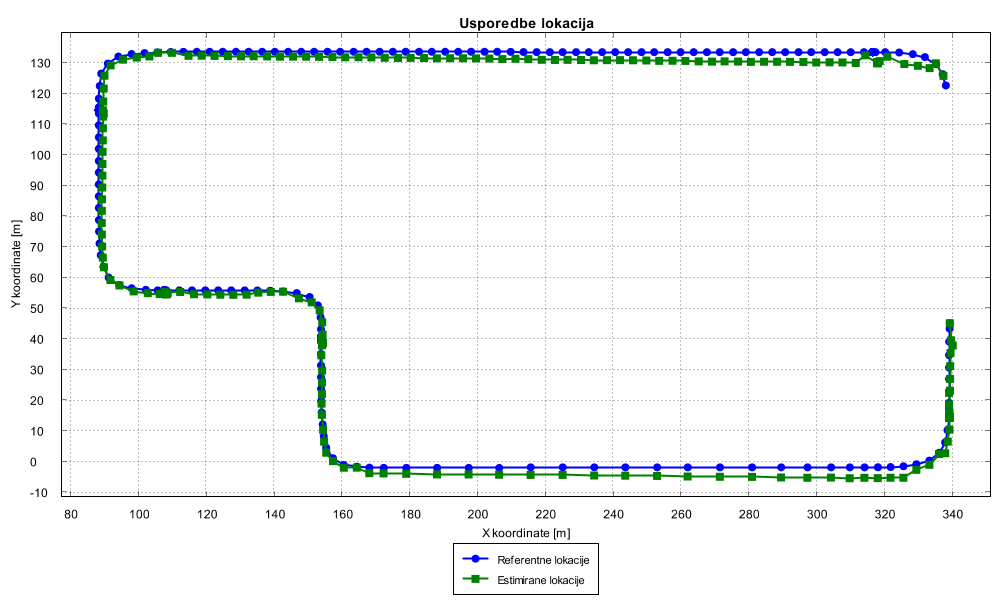
\includegraphics[scale=0.4]{images/algo1/primjer3/usporedba_lokacija.png}
  \caption{Graf lokacije vozila}
  \label{eval:a1p3_lokacija}
\end{figure}
